\documentclass{beamer}
\usetheme{Madrid}

\usepackage{amsmath, amssymb, amsthm}
\usepackage{graphicx}
\usepackage{listings}
\usepackage{gensymb}
\usepackage[utf8]{inputenc}
\usepackage{hyperref}
\usepackage{tikz}
\lstset{
  language=Python,
  basicstyle=\ttfamily\small,
  keywordstyle=\color{blue},
  stringstyle=\color{orange},
  numbers=left,
  numberstyle=\tiny\color{gray},
  breaklines=true,
  showstringspaces=false
}
\usetikzlibrary{decorations.pathmorphing}

\title{Question-9-9.3-13}
\author{EE24BTECH11030 - J.KEDARANANDA}
\date{}
\begin{document}

\frame{\titlepage}

\begin{frame}
\frametitle{Question}
Find the area bounded by the ellipse $x^2 + 4y^2 = 16$ and the ordinates $x = 0$ and $x = 2$.
\end{frame}

\begin{frame}
\frametitle{Inputs}

\centering
\begin{tabular}{ |c|c|}
    \hline
    \textbf{Variable} & \textbf{Description}\\ 
    \hline
    $\vec{x_1},\vec{x_2},\vec{x_3},\vec{x_4}$ & Intersection points\\
    \hline
    $\vec{h}$ & Point on the given line\\
    \hline
    $\vec{m}$ & Direction vector of given line\\
    \hline
    $A$ & Area of the region\\
    \hline
\end{tabular}
\end{frame}

\begin{frame}
\frametitle{Formulas}
\centering
\begin{tabular}{ |c|c|}
    \hline
    \textbf{Conic} & \textbf{Expression}\\ 
    \hline
    ellipse & $\vec{x}^\top\vec{V}\vec{x} + 2\vec{u}^\top\vec{x} + f = 0$\\
    \hline
    line & $\vec{x}=\vec{h}+\kappa\vec{m}$\\
    \hline
\end{tabular}
\end{frame}

\begin{frame}
\frametitle{Solution}
\begin{align}
\vec{V}&=\begin{pmatrix}\frac{1}{16} & 0\\0 & \frac{1}{4}\end{pmatrix}\\
\vec{u}&=\begin{pmatrix}0\\0\end{pmatrix}\\
f&=-1
\end{align}
For the given line $x=2$, the values of $\vec{h}$ and $\vec{m}$ are:
\begin{align}
\vec{h}&=\begin{pmatrix}2\\0\end{pmatrix}\\
\vec{m}&=\begin{pmatrix}0\\1\end{pmatrix}
\end{align}
\end{frame}

\begin{frame}
\frametitle{Solution}
The intersection points are:
\begin{align}
\vec{x_1} &= \begin{pmatrix}2\\\sqrt{3}\end{pmatrix}\\
\vec{x_2} &= \begin{pmatrix}2\\-\sqrt{3}\end{pmatrix}\\
\vec{x_3} &= \begin{pmatrix}0\\2\end{pmatrix}\\
\vec{x_4} &= \begin{pmatrix}0\\-2\end{pmatrix}
\end{align}
\begin{align}
y &= \pm \sqrt{4 - \frac{1}{4}x^2}
\end{align}
\end{frame}

\begin{frame}
\frametitle{Solution}
The area \( A \) between the curves from \( x = 0 \) to \( x = 2 \) is given by:
\begin{align}
A = 4 \int_0^2 \sqrt{1 - \frac{x^2}{16}} \, dx
\end{align}
Simplifying, we get:
\begin{align}
A = 2\sqrt{3} + \frac{4\pi}{3}
\end{align}
\end{frame}

\begin{frame}
\frametitle{Diagram}
\begin{figure}[!ht]
    \centering
    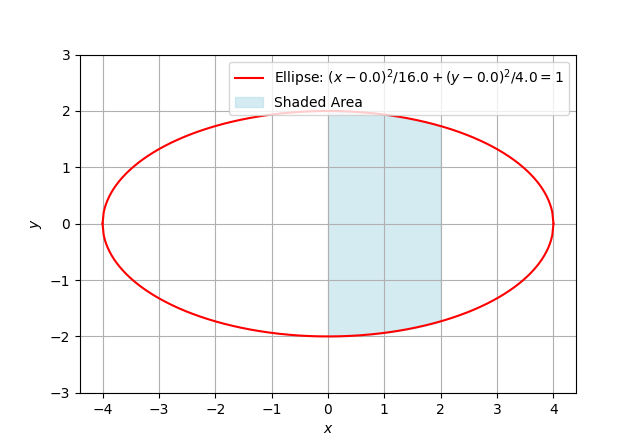
\includegraphics[width=\linewidth]{figs/fig1.png}
    \caption{Ellipse bounded region}
\end{figure}
\end{frame}

\begin{frame}[fragile]
\frametitle{C-Code}
\begin{lstlisting}[language=C]
#include <math.h>
#include <stdio.h>
#include <stdlib.h>
#include <string.h>
#include <unistd.h>
#include <sys/socket.h>
#include <netinet/in.h>

#include "libs/matfun.h"
#include "libs/geofun.h"

int main() {
    FILE *file;
    file = fopen("data.txt", "w");
\end{lstlisting}
\end{frame}
\begin{frame}[fragile]
\frametitle{C-Code}
    \begin{lstlisting}[language=C]
            if (file == NULL) {
        printf("Error opening file!\n");
        return 1; // Return error code if file couldn't be opened
    }
    // Ellipse parameters
    double a = 4.0; // semi-major axis
    double b = 2.0; // semi-minor axis
    // Store the parameters
    fprintf(file, "%lf\n%lf\n%lf\n%lf\n", a, b, 0.0, 0.0); // a, b, h, k
    fclose(file); // Close the file
    return 0; // Return success
}
    \end{lstlisting}
\end{frame}
\begin{frame}[fragile]
\frametitle{Python-Code}
\begin{lstlisting}
# Code by GVV Sharma
# Modified for Problem Solution
# Released under GNU GPL
# Calculating area enclosed between curves
import sys  # For path to external scripts
sys.path.insert(0, '/home/kedar/assignments/matgeo/codes/CoordGeo')  # Path to my scripts

import numpy as np
import matplotlib.pyplot as plt
from scipy.integrate import quad
\end{lstlisting}
\end{frame}

\begin{frame}[fragile]
\frametitle{Python-Code}
\begin{lstlisting}
# Read the values from the C-generated text file using numpy.loadtxt
try:
    data = np.loadtxt('data.txt')
except OSError:
    print("Error: Unable to read 'data.txt'. Please ensure the file exists.")
    sys.exit(1)

# Extracting ellipse parameters
a = data[0]  # semi-major axis
b = data[1]  # semi-minor axis
h = data[2]  # center x-coordinate (h)
k = data[3]  # center y-coordinate (k)
\end{lstlisting}
\end{frame}

\begin{frame}[fragile]
\frametitle{Python-Code}
\begin{lstlisting}
# Ellipse equations
def ellipse_upper(x, a, b, h, k):
    """Returns the upper part of the ellipse."""
    return k + b * np.sqrt(1 - ((x - h) * 2) / (a * 2))

def ellipse_lower(x, a, b, h, k):
    """Returns the lower part of the ellipse."""
    return k - b * np.sqrt(1 - ((x - h) * 2) / (a * 2))
\end{lstlisting}
\end{frame}

\begin{frame}[fragile]
\frametitle{Python-Code}
\begin{lstlisting}
# Define the limits of integration
x_min = 0
x_max = 2

# Compute the area between the curves using integration
def area_between_curves(x):
    """Calculates the difference between the upper and lower ellipse."""
    return ellipse_upper(x, a, b, h, k) - ellipse_lower(x, a, b, h, k)

# Perform the integration from x_min to x_max
area, _ = quad(area_between_curves, x_min, x_max)

print(f"Area enclosed between the ellipse and the ordinates: {area:.4f}")
\end{lstlisting}
\end{frame}

\begin{frame}[fragile]
\frametitle{Python-Code}
\begin{lstlisting}
# Visualization
# Generating points for the ellipse to show the complete ellipse
x_vals = np.linspace(h - a, h + a, 400)
y_upper = ellipse_upper(x_vals, a, b, h, k)
y_lower = ellipse_lower(x_vals, a, b, h, k)

# Plot the ellipse's upper and lower parts
plt.plot(x_vals, y_upper, label=f'Ellipse: $(x - {h})^2/{a*2} + (y - {k})^2/{b*2} = 1$', color='r')
plt.plot(x_vals, y_lower, color='r')
\end{lstlisting}
\end{frame}

\begin{frame}[fragile]
\frametitle{Python-Code}
\begin{lstlisting}
# Shade the area between the ellipse and the x-axis between x=0 and x=2
y_fill_upper = ellipse_upper(np.linspace(x_min, x_max, 100), a, b, h, k)
y_fill_lower = ellipse_lower(np.linspace(x_min, x_max, 100), a, b, h, k)

# Fill the area
plt.fill_between(np.linspace(x_min, x_max, 100), y_fill_upper, y_fill_lower, color='lightblue', alpha=0.5, label='Shaded Area')

# Labels and plot settings
plt.xlabel('$x$')
plt.ylabel('$y$')
plt.grid(True)
plt.legend(loc='upper right')
\end{lstlisting}
\end{frame}

\begin{frame}[fragile]
\frametitle{Python-Code}
\begin{lstlisting}
# Set the limits for y-axis to ensure complete visibility of the ellipse
plt.ylim(k - b - 1, k + b + 1)  # Slightly adjust as needed for aesthetics

# Set equal aspect ratio to avoid distortion
plt.gca().set_aspect('equal', adjustable='box')

# Show the plot
plt.show()
\end{lstlisting}
\end{frame}
\end{document}
